\chapter{Analiză și proiectare}

\section{Scenarii de utilizare}

Utilizatorul poate efectua următoarele acțiuni:
\subsection{Logare}
Utilizatorul se loghează în aplicație, care îl va redirecta către platforma Flickr, pentru a efectua autentificarea prin intermediul acesteia.

\subsection{Alege sursa imaginilor}
Utilizatorul poate alege sursa imaginilor ce vor fi analizare: propriul profil, imaginile contactelor sale, sau imagini publice de pe platforma Flickr.

\subsection{Încarcă imagine}
Pentru a efectua această acțiune, utilizatorul trebuie să fi trecut prin pasul de logare și eventual să fi ales sursa imaginilor. Dacă acesta nu a ales sursa imaginilor, în mod implicit aceasta este propriul profil. Scenariul acesta de utilizare presupune ca utilizatorul să aleagă o imagine de pe propriul dispozitiv pe care să o trimită către aplicație.

Pentru a returna imaginile similare din punct de vedere vizual, aplicația va efectua următoarele acțiuni:
\begin{enumerate}
    \item Analizează imaginea încărcată folosind o rețea neurală și returnează o serie de etichete descriptive
    \item Aduce imaginile  din sursa selectată de utilizator
    \item Analizează imaginile aduse, obținând pentru fiecare o serie de etichete
    \item Descoperă similaritatea între imagini comparând etichetele și obține o listă de imagini corespunzătoare
    \item Afișează imaginile din lista obținută
\end{enumerate}{}

 \begin{figure}[!htbp]
    \begin{center}
        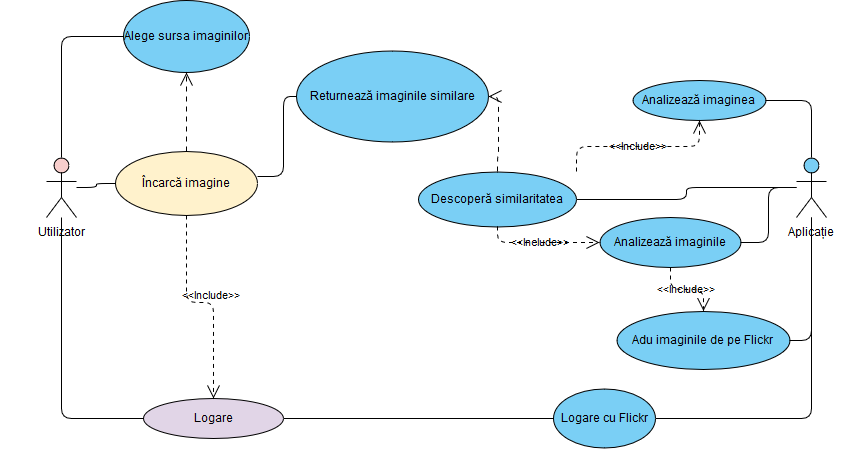
\includegraphics[width=0.9\textwidth]{images/use_case.png}
        \caption{Diagrama de scenarii de utilizare a aplicației}
    \end{center}
\end{figure}


\section{Arhitectura aplicației}
Aplicația este împărțită în două module, dar folosește și anumite servicii externe.Utilizatorul interacționează direct cu modulul  \textit{front-end}, o aplicație web realizată cu ajutorul \textit{framework}-ului Angular în limbajul Typescript. La rândul său, modulul este împărțit în mai multe componente, acestea apelând unele servicii. Modulul de back-end este realizat cu ajutorul \textit{framework}-ului Flask în limbajul Python. Se folosesc mai multe biblioteci pentru a efectua anumite operații(ex. \textit{requests} pentru a apela API-uri, \textit{pony.orm} pentru conectarea la baza de date) și \textit{framework}-uri specializate pentru rețele neuronale(Tensorflow și Keras). Serviciile externe sunt reprezentate de API-urile platformelor Flickr(pentru autentificare, informații despre profil și imagini) și DataMuse(pentru a obține sinonime). De asemenea se mai folosește o bază de date SQLite pentru reținerea \textit{token}-ului de acces și identificatorului unic.

 \begin{figure}[!htbp]
    \begin{center}
        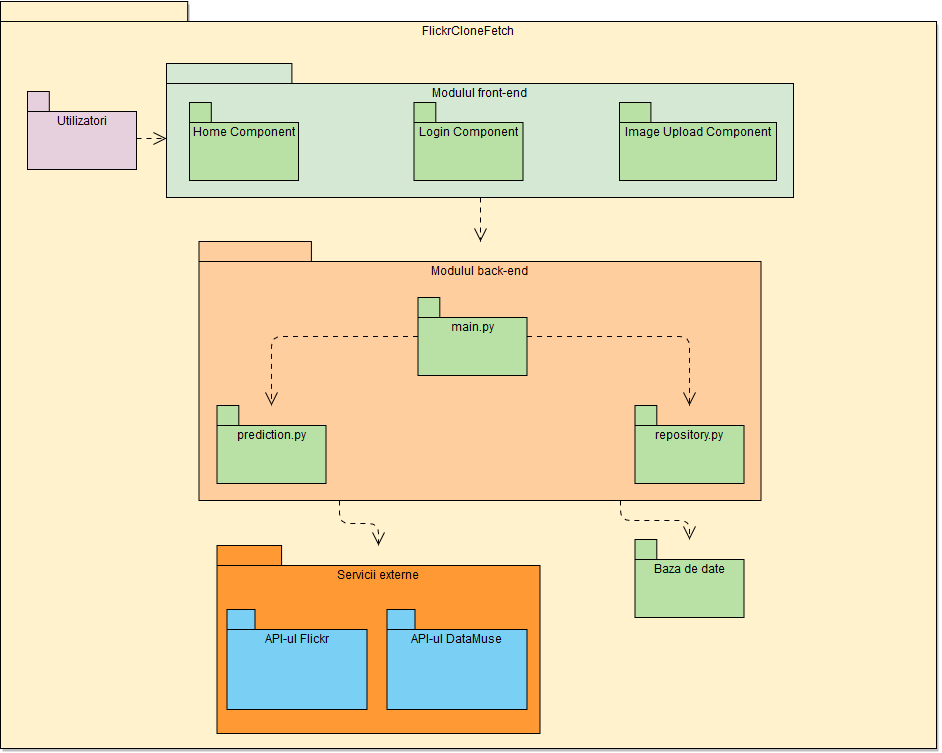
\includegraphics[width=1.0\textwidth]{images/arhitectura.png}
        \caption{Arhitectura aplicației}
    \end{center}
\end{figure}

\section{Planificarea activităților realizate de către aplicație}
Fluxul de activități în cadrul aplicației se desfășoară în modul urmator
\begin{enumerate}
    \item Modulul \textit{front-end} afișează pagina de logare și redirectează utilizatorul la procesul de logare de pe \textit{back-end} (Home Component)
    \item Modulul \textit{back-end} trimite cererea de logare prin OAuth la API-ul Flickr
    \item  Se salvează \textit{request token}-ului și redirectarea la autorizarea pagina de logare în Flickr și autorizare prin API-ul Flickr
    \item Se trimite \textit{request token}-ul autorizat de către utilizator pentru a obține un \textit{token} de acces
    \item  Se generează un identificator unic pentru utilizator, se salvează în baza de date împreună cu \textit{token}-ul de acces primit și apoi se face redirectarea către \textit{front-end} trimițând și identificatorul unic
    \item Modulul \textit{front-end} reține identificatorul utilizatorului și cere  datele despre profil 
    \item Modulul \textit{back-end} furnizează datele despre profil(nume utilizator, imagine de profil)
    \item \textit{Front-end}-ul redirectează utilizatorul la pagina de încărcare imagini (Login Component)
    \item Aici i se oferă utilizatorului posibilitatea de a încărca o imagine și de a alege sursa imaginilor, apoi trimite la modulul \textit{back-end} aceste informații (Image Upload Component)
    \item Modulul \textit{back-end} primește imaginea și opțiunile privitoare la sursă și  analizează imaginea cu o rețea neurală, obținând o listă de etichete
    \item Se apelează API-ul DataMuse pentru a obține cuvinte similare etichetelor obținute
    \item Se apelează API-ul Flickr pentru a obține imagini și acestea se  analizează cu rețeaua neurală
    \item Se compară etichetele imaginilor cu etichetele imaginii încărcate și se creează o listă de imagini similare
    \item Se returnează lista către \textit{front-end}
    \item \textit{Front-end}-ul afișează imaginile returnate de \textit{back-end} (Image Upload Component)
\end{enumerate}{}

\begin{figure}[!htbp]
    \begin{center}
        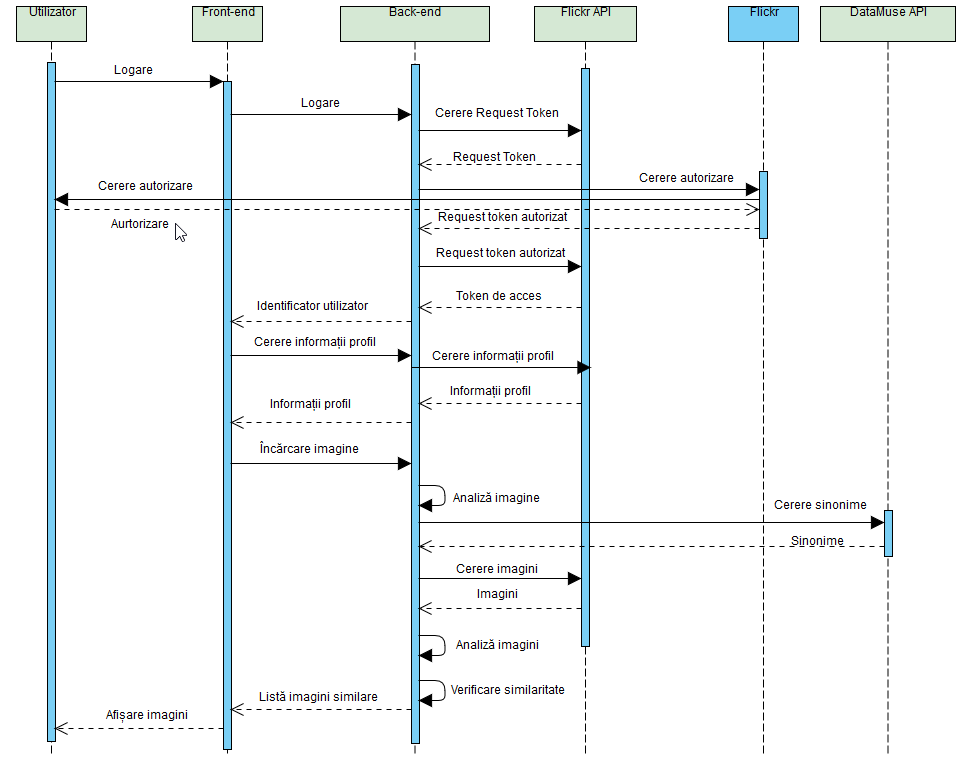
\includegraphics[width=1.0\textwidth]{images/secventa.png}
        \caption{Diagrama de secvență a aplicației}
    \end{center}
\end{figure}

\section{Modulul \textit{back-end}}

\subsection{API-ul expus}
Specificația OPENApi a API-ului se găsește la ~\nameref{ch:anexa1}
\subsubsection{/login}
Endpoint pentru logare, utilizatorul este redirectat aici de către modulul \textit{front-end}. Aplicația va redirecta la rândul ei catre /authorize.

\subsubsection{/authorize}
Endpoint pentru autorizare, se ajunge aici din redirectarea efectuată de către aplicație. Are ca parametrii \textit{oauth-token} și \textit{oauth-verifier} și va redirecționa către \textit{front-end}.

\subsubsection{/profile}
Returnează informațiile despre profilul de Flickr al utilizatorului: numele utilizatorului și imaginea sa de profil. Are ca parametru identificatorul utilizatorului.

\subsubsection{/addImage}
Primește identificatorul utilizatorului, imaginea în base64 și opțiunea privitoare la sursa imaginilor ce vor fi analizate. Returnează lista de etichete a imaginii și lista de imagini similare din punct de vedere vizual.

\subsection{Rețeaua neurală folosită}
Rețeaua neurală folosită pentru analiza imaginilor este un model numit \textit{NASNet Mobile}, obținut de Google prin \textit{framework}-ul NAS(Neural Architecture Search) și discutat în lucrarea \textit{Learning Transferable Architectures for Scalable Image Recognition}. \cite{DBLP:journals/corr/ZophVSL17}

Proiectul \textit{AutoML}, prin \textit{framework}-ul NAS, propune următorul lucru: o rețea neurală controler propune o arhitectură de rețea "copil" care va fi antrenată și evaluată pe o anumită sarcină. Evaluarea este folosită pentru a calibra rețeaua controler, care va propune idei îmbunătățite de arhitectură la iterația următoare. Procesul se repetă de mii de ori, generând noi arhitecturi , testându-le și evaluându-le până când se obțin arhitecturi de rețele neurale noi utile.\cite{45826}

\begin{figure}[!htbp]
    \begin{center}
        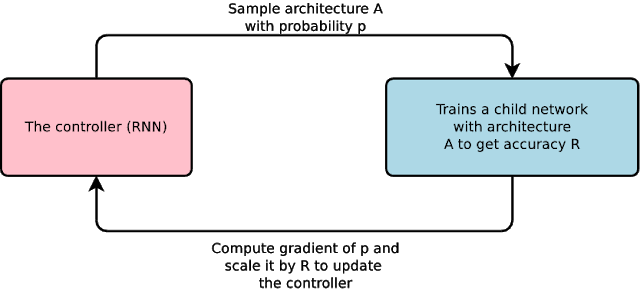
\includegraphics[width=0.6\textwidth]{images/nas.png}
        \caption{Procesul de obținere a noi rețele neurale folosind NAS \cite{45826}}
    \end{center}
\end{figure}

Arhitectura \textit{NASNet} este obținută prin procesul descris mai sus, cu unele mic modificări. Scopul rețelei e să clasifice imagini, deci a fost evaluată performanța pe doua din cele mai cunoscute seturi de date în mediul academic: setul de detecție de obiecte \textit{COCO} și setul de clasificare de imagini \textit{ImageNet}. Deoarece seturile acestea de date sunt foarte mari, AutoML a fost reprogramat să caute straturi care ar fi atunci când sunt conectate în număr mare. Căutarea straturilor a avut loc pe un set de date mai mic, CIFAR10, apoi cea mai bună arhitectură a fost scalată și transferată pentru antrenamentul pe COCO și ImageNet.\cite{DBLP:journals/corr/ZophVSL17}



\begin{figure}[!htbp]
    \begin{center}
        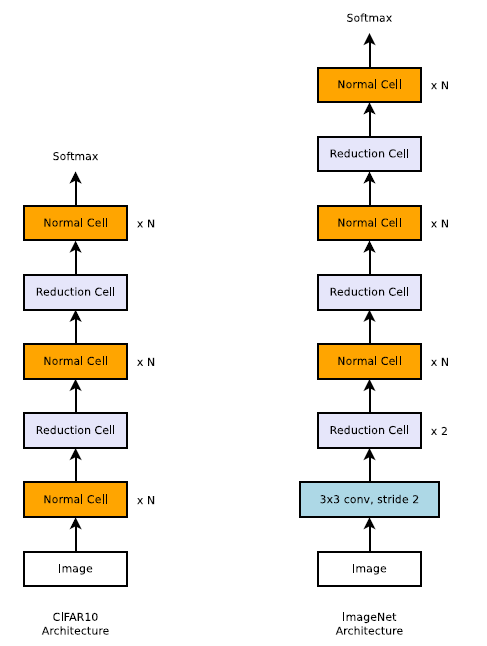
\includegraphics[width=0.75\textwidth]{images/nasnet.png}
        \caption{Arhitectura NASNet \cite{DBLP:journals/corr/ZophVSL17}}
    \end{center}
\end{figure}
Arhitectura \textit{NASNet} a fost predefinită, având două tipuri de straturi:
\begin{enumerate}
    \item \textit{Normal Cell} - un strat convoluțional care returnează o mapare de aceași dimensiune a imaginii
    \item \textit{Reduction Cell} - un strat convoluțional care reduce dimensiunea mapării cu un factor de doi
\end{enumerate}{}
Rețeaua neurală controler a trebuit doar să descopere cea mai bună arhitectură pentru cele două tipuri de straturi.

După aproximativ 4 zile de căutări au fost obținute mai multe arhitecturi de straturi candidat, care combinate produc arhitecturi cu rezultate comparabile cu alte arhitecturi din domeniu. Cele mai bune 3 arhitecturi obținute se numesc \textit{NASNet-A}, \textit{NASNet-B} și \textit{NASNet-C}.

\begin{figure}[!htbp]
    \begin{center}
        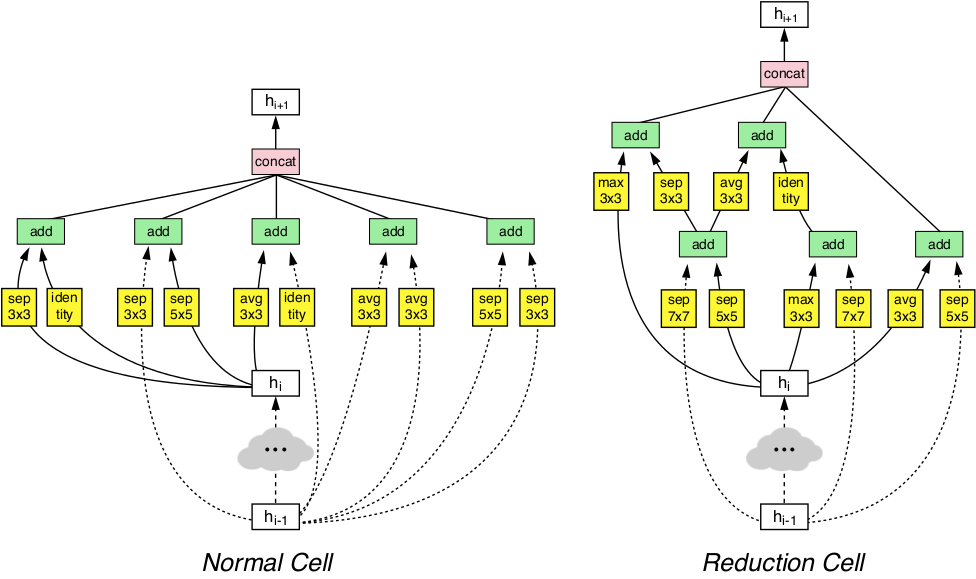
\includegraphics[width=1.0\textwidth]{images/nasnetcells.png}
        \caption{Celulele arhitecturii NASNet-A \cite{DBLP:journals/corr/ZophVSL17}}
    \end{center}
\end{figure}

Modelul folosit în aplicația {\applicationtitle}, numit \textit{NASNet Mobile}, este o versiune scalată a arhitecturii \textit{NASNet}, mai mică, cu 5 326 716 parametrii optimizată pentru un const computațional redus și o viteză mai mare. Modelul folosit este pre-antrenat pe 1000 de categorii din setul de date ImageNet, având o acuratețe de 91.9 procente pe același set de date.

\subsection{Baza de date}
Baza de date folosită, de tip SQLite, are un singur tabel folosit pentru a stoca \textit{token}-ul de acces și identificatorul unicat generat în relație cu acesta.

\begin{figure}[!htbp]
    \begin{center}
        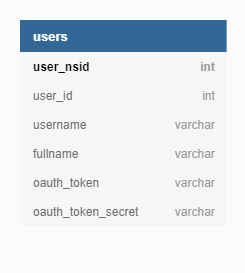
\includegraphics[width=0.4\textwidth]{images/database.png}
        \caption{Schema bazei de date folosite}
    \end{center}
\end{figure}